
\begin{columns}
\column{0.35\textwidth}
\centering
\begin{figure}
  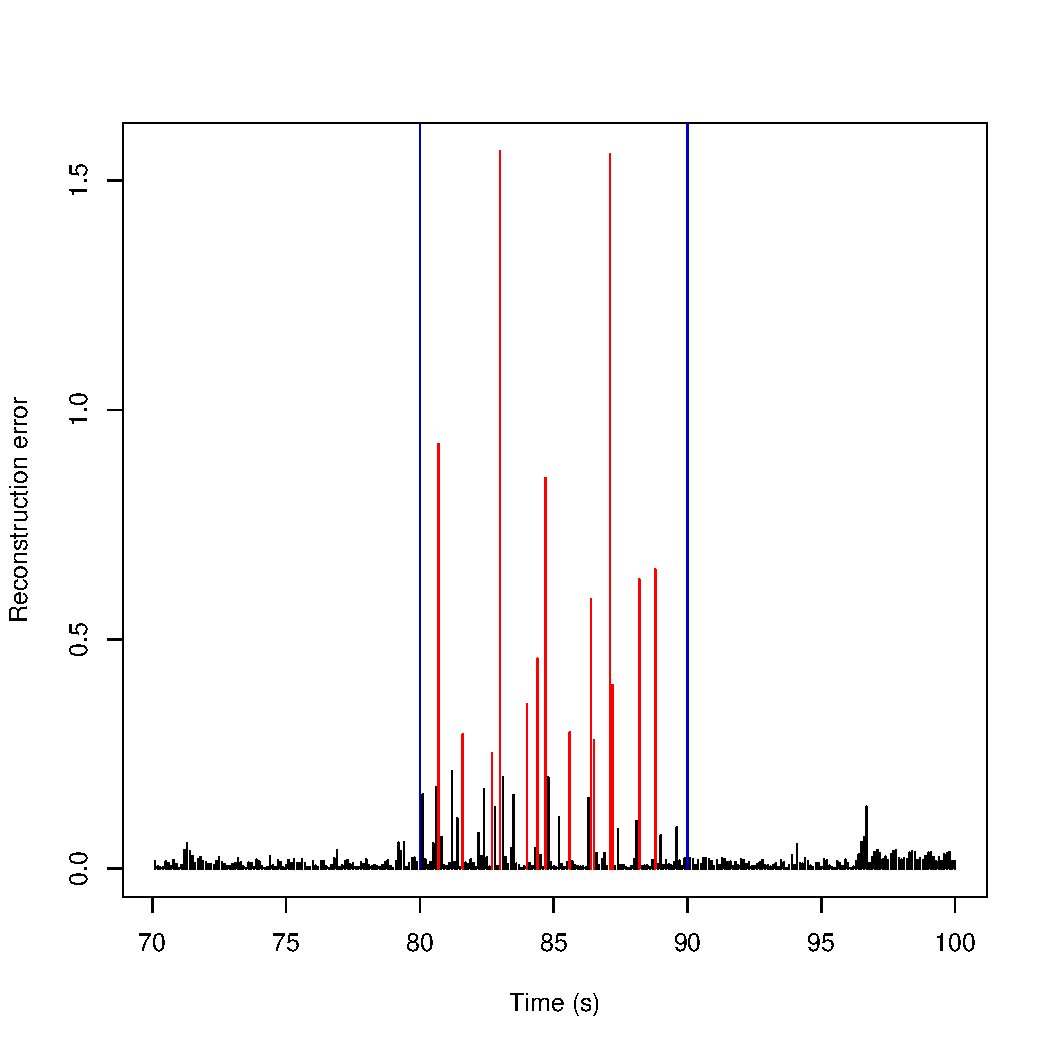
\includegraphics[width=\linewidth]{anomaly_detection_lorenz}
  \small
Error de reconstrucción en test (entre 80 y 90 s hay anomalías)
\end{figure}
\column{0.65\textwidth}
\scriptsize
\begin{Shaded}
\begin{Highlighting}[]
\NormalTok{reconstructions <-}\StringTok{ }\KeywordTok{autoencoder_denoising}\NormalTok{(}
  \KeywordTok{input}\NormalTok{() }\OperatorTok{+}
  \KeywordTok{dense}\NormalTok{(}\DecValTok{16}\NormalTok{, }\DataTypeTok{activation =} \StringTok{"sigmoid"}\NormalTok{) }\OperatorTok{+}
  \KeywordTok{output}\NormalTok{(), }
  \DataTypeTok{loss =} \StringTok{"mean_squared_error"}\NormalTok{, }
  \DataTypeTok{noise_type =} \StringTok{"saltpepper"}\NormalTok{, }\DataTypeTok{p =} \FloatTok{0.1}\NormalTok{) }\OperatorTok{\%>\%}
  \KeywordTok{train}\NormalTok{(x_train, }\DataTypeTok{epochs =} \DecValTok{50}\NormalTok{, }
    \DataTypeTok{batch_size =} \DecValTok{32}\NormalTok{)}\OperatorTok{ \%>\%}\StringTok{ }\KeywordTok{reconstruct}\NormalTok{(x_test)}

\NormalTok{errors <-}\StringTok{ }\KeywordTok{rowMeans}\NormalTok{(}
  \NormalTok{(reconstructions }\OperatorTok{-}\StringTok{ }\NormalTok{x_test) }\OperatorTok{**}\StringTok{ }\DecValTok{2}\NormalTok{)}
\end{Highlighting}
\end{Shaded}\normalsize
\end{columns}
